\documentclass[runningheads]{llncs}

\usepackage{graphicx}
\usepackage{amsmath}
\usepackage{amssymb}
\usepackage{booktabs}
\usepackage{multirow}
\usepackage{array}
\usepackage{url}
\usepackage{algorithm}
\usepackage{algorithmic}
\usepackage{subcaption}
\usepackage{mdframed}
\usepackage{hyperref}
\usepackage{tikz}
\usepackage{pgfplots}
\usepackage{float}
\pgfplotsset{compat=1.18}

\bibliographystyle{splncs04}

\begin{document}

\title{Emotional Models: Text Mood Classification}
\author{
    Miguel Cabral Pinto\inst{1} \and Tiago Silva\inst{2} \\
    \email{\inst{1}mcp@student.uc.pt, \inst{2}tds@student.uc.pt}
}
\authorrunning{M. Cabral Pinto \and T. Silva}
\institute{
    Department of Informatics Engineering \\ University of Coimbra \\ Coimbra, Portugal\\
}

\maketitle

\begin{abstract}
    This project explores the classification of emotional states in text using supervised and zero-shot learning approaches. 
    We implement and compare artificial neural networks (ANNs) and transformer-based models to categorize text into six emotion classes. 
    The methodology includes training ANNs for various epochs and evaluating their performance using confusion matrices and accuracy metrics. 
    Additionally, we assess large pre-trained BERT models in a zero-shot setting, in order to draw comparisons between the two approaches. 
    Experimental results demonstrate the effectiveness of both supervised and zero-shot models, with comparative analysis highlighting their strengths and limitations for these sorts of tasks.

    \keywords{Emotion Classification \and Supervised Learning \and Zero-shot Learning \and BERT \and Artificial Neural Networks}
\end{abstract}

\section{Methodology}

\subsection{Dataset}

For the purpose of classifying emotional states in text, we utilize the dataset requested in the project statement (HuggingFace's \texttt{dair-ai/emotion}\footnote{\url{https://huggingface.co/datasets/dair-ai/emotion}}), consisting of labeled examples across six emotion categories: sadness, joy, love, anger, fear, and surprise.
The characteristics of its split version, which will be used in this project, are as follows:

\begin{itemize}
    \item \textbf{Source:} Social media (Twitter) messages
    \item \textbf{Language:} English
    \item \textbf{Text Length:} 7 \textrightarrow~300 characters
    \item \textbf{Classes:} 6 (sadness, joy, love, anger, fear, surprise)
    \item \textbf{Training Set:} 16000 labeled examples
    \item \textbf{Validation Set:} 2000 labeled examples
    \item \textbf{Test Set:} 2000 labeled examples
    \item \textbf{Total:} 20000 labeled examples
\end{itemize}

\begin{figure}[H]
    \centering
    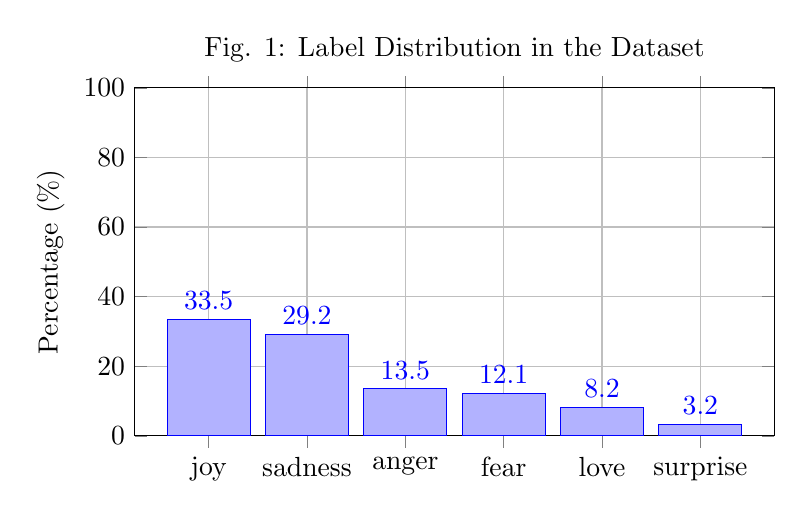
\begin{tikzpicture}
        \begin{axis}[
            ybar,
            bar width=30pt,
            width=0.8\textwidth,
            height=6cm,
            ymin=0,
            ymax=100,
            xtick=data,
            xticklabels={joy, sadness, anger, fear, love, surprise},
            ylabel={Percentage (\%)},
            title={Fig. 1: Label Distribution in the Dataset},
            nodes near coords,
            nodes near coords align={vertical},
            enlarge x limits=0.15,
            grid=major,
        ]
        \addplot coordinates {(0,33.5) (1,29.2) (2,13.5) (3,12.1) (4,8.2) (5,3.2)};
        \end{axis}
    \end{tikzpicture}
    \label{fig:label_distribution}
\end{figure}
\vspace{-0.5cm}

\noindent Upon initially looking at the data, a challenge immediately became apparent: class imbalance. 
Rarer emotions are heavily misrepresented (only 3.2\% of examples have a ``surprise'' label), while simpler, more common emotions which may overlap with others dominate the dataset (the ``joy'' and ``sadness'' classes hold a joint 62.7\% of the examples).
This is an issue because the model can specialize in a subset of the classes and be biased towards them.
In this case, completely ignoring ``surprise'' but getting every other example right would give the model a misleadingly high accuracy of approximately 96.8\%.
This is one of the reasons why accuracy alone is not a sufficient metric for evaluating model performance in this context, and why confusion matrices and other metrics computed from them (particularly those that measure per-class performance) are very important.
This dataset imbalance has other implications as well, specially when comparing two diferent paradigms (supervised learning and zero-shot classification), as each may be affected differently by the lack of data for certain classes.
On the one hand we have the ANNs which are directly harmed by the lack of class representation because they learn from the empirical distribution of the data, affecting the decision boundaries they create. 
On the other hand we have the zero-shot models which dont learn from the data, contrastingly they may be less affected by class imbalance, but their performance may still vary across classes due to the inherent biases in the pre-trained models they rely on.

\noindent Another problem that stands out when analyzing the data is the reliability of its labels.
Several of the data points show text-label pairs with a mismatch that is obvious to a human eye, with the most common pattern being lack of context undestanding.
For example, texts like \textit{i no longer feel happy to score well} and \textit{i never feel that popular} were both labeled as ``joy'' due to their use of \textit{happy} and \textit{popular}, words that usually convey positive emotions, even though in these cases their negation is used, causing the overall sentiment to be reversed.
Inconsistencies such as these mean that there is a cap to the performance of any model on this dataset, unless it overfits to the noise in the labels (even then, it is not guaranteed that the training and testing sets will have the same types of mismatches).
This is shown by Kermani et al.\cite{kermani2025systematicevaluationllmstrategies} as their attempt at fine-tuning an extensive model (LLaMA-38B) for this task achieves the best performance out of the tried approaches (including zero-shot classification, which is explored in this project) at 91\%.

\noindent In order to understand the dataset better, it is important to consider how it was populated.
Though no information is provided in the HuggingFace website on this aspect, the GitHub repository containing the data\footnote{\url{https://github.com/dair-ai/emotion_dataset}} links to a paper by the authors that details the creation process \cite{saravia-etal-2018-carer} (though the repository and paper do not refer to the same dataset, they are populated in the same manner).
The proposed model, CARER, consists of a semi-supervised, graph-based algorithm designed to create contextualized emotion representations that relies on \textit{enriched patterns}, which identify similar text structures across examples to help with classification.
However, our manual analysis suggests that while the CARER method aims to account for context, its application in creating this specific dataset may not have fully overcome the challenge of syntactic nuance, leaving a pattern of keyword-emotion association in some entries.

\subsection{Implementation}
The main goal of this project is to explore and compare supervised and zero-shot learning approaches for emotion classification using a modular and reproducible experimental setup.
It is implemented in Python and organized into modular scripts to facilitate experimentation.

\noindent The supervised learning pipeline is defined in \texttt{supervised.py}, which is an adaptation of the code initially provided with this assignment, where artificial neural networks (ANNs) are constructed and trained using the dataset. 
The script relies on PyTorch for model definition, training, and evaluation. 
Training progress and results, including confusion matrices and accuracy metrics, are logged for analysis. 
The main orchestration of experiments, including data loading, model selection, and evaluation, is handled in \texttt{main.py}.

\noindent For zero-shot classification, \texttt{zero\_shot.py} utilizes transformer models from the HuggingFace library, such as BERT.
It differs from the previous approach by performing data point classification without explicit training on the dataset labels, instead infering emotions directly from text using pre-trained language representations.

\noindent Supporting modules include \texttt{metrics.py}, which provides functions for computing evaluation metrics such as accuracy, F1-score and comparative analysis utilities. Beyond basic metrics, we implement specialized analysis functions in \texttt{metrics.py}:
\begin{itemize}
    \item \texttt{compare\_supervised\_configs}: Tracks the evolution of per-class recall, specificity, and precision across different training epochs (5, 10, 20), identifying which emotions benefit from longer training and which plateau or degrade (potential overfitting).
    \item \texttt{extract\_top\_confusions}: Identifies the most frequent misclassification patterns globally, revealing systematic errors (e.g., confusing ``love'' with ``joy'', which accounts for 34.6\% of ``love'' misclassifications).
    \item \texttt{analyze\_class\_mistakes}: Analyzes confusions for individual classes, showing which emotions are most often misclassified as a given target emotion.
\end{itemize}
Finnaly, we log all experimental results and configurations using \texttt{logs.py} for the consequent analysis and comparison of different models and settings.
% \begin{table}[ht]
%     \centering
%     \caption{Confusion Matrix for 6-Class Classification}
%     \begin{tabular}{c|cccccc}
%         \toprule
%         \textbf{ Pred. / Real } & \textbf{ sadness} & \textbf{joy} & \textbf{love} & \textbf{anger} & \textbf{fear} & \textbf{surprise} \\
%         \midrule
%         \textbf{sadness }   &  &  &  &  &  &  \\
%         \textbf{joy}       &  &  &  &  &  &  \\
%         \textbf{love}      &  &  &  &  &  &  \\
%         \textbf{anger}     &  &  &  &  &  &  \\
%         \textbf{fear}      &  &  &  &  &  &  \\
%         \textbf{surprise }  &  &  &  &  &  &  \\
%         \bottomrule
%     \end{tabular}
%     \label{tab:confusion_matrix}
% \end{table}

% \begin{table}[ht]
%     \centering
%     \caption{ANN Confusion Matrix (5 epochs, acc=0.6980)}
%     \begin{tabular}{c|cccccc}
%         \toprule
%         \textbf{ Pred. / Real } & \textbf{ sadness} & \textbf{joy} & \textbf{love} & \textbf{anger} & \textbf{fear} & \textbf{surprise } \\
%         \midrule
%         \textbf{sadness}   & 418 & 72  & 8  & 39  & 40  & 4  \\
%         \textbf{joy}        & 36  & 574 & 33 & 26  & 22  & 4  \\
%         \textbf{love}       & 13  & 78  & 58 & 8   & 2   & 0  \\
%         \textbf{anger}      & 36  & 40  & 4  & 179 & 16  & 0  \\
%         \textbf{fear}       & 28  & 27  & 1  & 13  & 147 & 8  \\
%         \textbf{surprise}  & 7   & 20  & 1  & 4   & 14  & 20 \\
%         \bottomrule
%     \end{tabular}
%     \label{tab:cm_ann_5}
% \end{table}

% \begin{table}[ht]
%     \centering
%     \caption{ANN Confusion Matrix (10 epochs, acc=0.7190)}
%     \begin{tabular}{c|cccccc}
%         \toprule
%         \textbf{ Pred. / Real } & \textbf{ sadness} & \textbf{joy} & \textbf{love} & \textbf{anger} & \textbf{fear} & \textbf{surprise } \\
%         \midrule
%         \textbf{sadness}   & 470 & 49  & 13 & 16  & 26  & 7  \\
%         \textbf{joy}       & 55  & 537 & 49 & 20  & 27  & 7  \\
%         \textbf{love}      & 15  & 57  & 77 & 5   & 4   & 1  \\
%         \textbf{anger}     & 62  & 32  & 7  & 154 & 19  & 1  \\
%         \textbf{fear}      & 29  & 18  & 2  & 9   & 156 & 10 \\
%         \textbf{surprise}  & 8   & 15  & 2  & 3   & 12  & 26 \\
%         \bottomrule
%     \end{tabular}
%     \label{tab:cm_ann_10}
% \end{table}

% \begin{table}[ht]
%     \centering
%     \caption{ANN Confusion Matrix (20 epochs, acc=0.7290)}
%     \begin{tabular}{c|cccccc}
%         \toprule
%         \textbf{ Pred. / Real } & \textbf{ sadness} & \textbf{joy} & \textbf{love} & \textbf{anger} & \textbf{fear} & \textbf{surprise } \\
%         \midrule
%         \textbf{sadness}   & 469 & 50  & 10 & 27  & 20  & 5  \\
%         \textbf{joy}       & 51  & 550 & 40 & 24  & 21  & 9  \\
%         \textbf{love}      & 17  & 54  & 76 & 9   & 2   & 1  \\
%         \textbf{anger}     & 43  & 29  & 5  & 187 & 11  & 0  \\
%         \textbf{fear}      & 32  & 17  & 2  & 14  & 149 & 10 \\
%         \textbf{surprise}  & 8   & 16  & 1  & 3   & 11  & 27 \\
%         \bottomrule
%     \end{tabular}
%     \label{tab:cm_ann_20_new}
% \end{table}

% \begin{table}[ht]
%     \centering
%     \caption{ModernBERT-large-zeroshot-v2.0 CM (acc=0.7250)}
%     \begin{tabular}{c|cccccc}
%         \toprule
%         \textbf{ Pred. / Real } & \textbf{ sadness} & \textbf{joy} & \textbf{love} & \textbf{anger} & \textbf{fear} & \textbf{surprise } \\
%         \midrule
%         \textbf{sadness}   & 431 & 69  & 16 & 28  & 34  & 3  \\
%         \textbf{joy}       & 42  & 571 & 39 & 13  & 21  & 9  \\
%         \textbf{love}      & 14  & 67  & 67 & 6   & 3   & 2  \\
%         \textbf{anger}     & 25  & 27  & 4  & 191 & 19  & 9  \\
%         \textbf{fear}      & 25  & 10  & 1  & 9   & 165 & 14 \\
%         \textbf{surprise}  & 7   & 21  & 1  & 2   & 10  & 25 \\
%         \bottomrule
%     \end{tabular}
%     \label{tab:cm_ann_20_new}
% \end{table}

% \section{Methodology}

% \subsection{Dataset}

% \section{Results}

% \subsection{Comparative Analysis}
% a

% \section{Conclusion}
% A

\newpage % during development!
\bibliography{references}

\end{document}
